\documentclass[12pt]{article}

\usepackage{amsfonts}
\usepackage{amsmath}
\usepackage{graphicx}
\usepackage{lmodern}
\usepackage{hyperref}

\title{Ardana Rollups System Architecture}
\author{Ardana Labs}


\begin{document}


\maketitle


Ardana Rollups are a general purpose ZK rollup layer 2 scalability solution for Cardano. ZK rollups are a mechanism by which transactions are processed off-chain and the results of those transactions are published onto the blockchain using zero knowledge proofs. More precisely, ZK rollups use zkSNARKS, which are in other words zero knowledge succinct non-interactive arguments of knowledge. By moving data and processing off-chain, ZK rollups allow for higher throughput. By using a secure, decentralized layer 1 blockchain and zkSNARKS, ZK rollups inherit certain security properties of the layer 1 solution, namely that we need not assume that any party is trustworthy, and nobody is able to violate the protocol and cause incorrect results to be produced on-chain. Additionally, Ardana Rollups are designed to have the security property that there is no single point of failure, meaning that there is no individual or organization whose ongoing participation is required for the proper, intended functioning of the solution.

ZK rollups are an increasingly popular choice of layer 2 solution on Ethereum, with multiple choices of ZK rollup solution available for use, including zkSync, StarkEx, and Loopring. \cite{ethworks-20} In contract, we know of no prior art for a ZK rollup based layer 2 solution on Cardano. However, we believe that ZK rollups will be an important part of the Cardano ecosystem moving forward, just as they are in Ethereum today.

This is the system architecture document for Ardana Rollups. This defines the key components of Ardana Rollups and their interactions with each other and the outside world, as well as the rationale for those design decisions. This is different from a whitepaper or a technical spec in that it does not attempt to provide enough information to implement Ardana Rollups. Instead, you can think of it as a sketch. Technical specs will fill in the picture in much greater detail, sufficient to guide implementation, and a technical whitepaper will describe Ardana Rollups in a form more suitable for general consumption.

\section{Background}

This section covers background information necessary to understand the design of Ardana Rollups and ZK rollup solutions more generally.

A blockchain uses a consensus algorithm executed by a decentralized network of nodes in order to process financial transactions and other information. Thanks to the consensus algorithm, parties can be assured that their money and other information assets stored on the blockchain will not be used in a manner they did not authorize, without a need to trust that any particular participant in the protocol is behaving honestly.

Blockchains are an important innovation in financial technology which have the potential to liberate humanity from centralized systems of finance. However, this will only be possible to the extent that blockchain developers can obtain massive scalability, such that these systems could actually replace the centralized financial technology which most people use most of the time to settle financial transactions electronically today. For example, Visa reportedly processes over 150 million transactions per day on average, and is capable of processing more than 24,000 transactions per second. \cite{visa}

Scalability of blockchain solutions is a widely recognized problem. There are a few angles of attack on this problem. One angle is to increase the transaction throughput of the blockchain itself. This is an important task but also a difficult one. Another angle is to multiply the number of blockchains in use, such as in the case of Kadena's Chainweb. \cite{chainweb} A third angle is to use so-called layer 2 solutions, whereby transactions are processed off-chain and then the results are later synced onto the chain. With layer 2 solutions, the blockchain can be used simply as a settlement layer, while application domain business logic lives off-chain and the amount of state and state changes stored on the chain can be greatly reduced.

ZK rollups are an example of a layer 2 solution strategy. ZK rollups make use of zkSNARKs. zkSNARKs are a type of proof. A proof, for our purposes, is a piece of information which evidences the truth of some statement. In the context of formal logic, a proof is in other words a sound argument, which is a valid argument where the premises are true. A valid argument, speaking informally, is an argument which in virtue of its logical structure guarantees that the conclusion is true provided that the premises are true. This is \emph{not}\/ what we mean by a proof here. A proof in this context is a piece of information whose existence demonstrates that there is only a negligible probability that the statement to be proven is not true. In this sense of the word proof, for example, an ED25519 signature is a proof that a person who has the private signing key ran the signing algorithm on the piece of information that was signed.

By definition, a zkSNARK is a zero knowledge succinct non-interactive argument of knowledge. In this definition, ``argument of knowledge'' means ``proof'' (in the sense of ``proof'' just stated). A zkSNARK has the characteristics of being zero knowledge (meaning it does not prove anything more than the statement to be proven), succinct (meaning the proof can be represented as a small number of bytes), and non-interactive (meaning the proof can be represented as a single message, as opposed to a multi-step interaction between the proving entity and proof-checking entity).

For our purposes, the most relevant characteristics of zkSNARKs are the succinct and non-interactive properties. It may be the case that we could get by with just SNARKs, i.e., succinct non-interactive proofs which are not necessarily zero-knowledge. However, we are using zkSNARKs for the reason that the bulk of the research on SNARKs is on zkSNARKs, and we believe that the most mature SNARK solutions available are zkSNARK solutions.

The reason that succinctness and non-interactivity are key properties here is that we need to store the proofs in transactions on the blockchain. Thus due to the nature of blockchain transactions, which are short single messages, the proofs must be succinct and non-interactive.

ZK rollups are in essence a simple concept. In a pure blockchain protocol (without a layer 2 solution), we store all transactions, all smart contract code, and all smart contract state data on the blockchain. In a ZK rollup solution, we move some of this code and data off-chain, and instead we store on the chain proofs that this information exists. The zkSNARKs stored on chain prove that for some set of inputs and some set of outputs, there exists a set of transactions which were signed by the relevant parties and which followed the rules of the relevant smart contracts. Those transactions never need to be recorded on the chain; we need only record the inputs, the outputs, and the proof that those outputs lawfully (according to the laws of the blockchain protocol) resulted from the inputs.

Due to the nature of zkSNARKs, this strategy allows for a potentially unlimited number of transactions to be performed with a constant $O(1)$ amount of on-chain information. Therefore this ZK rollup strategy allows for potentially very efficient usage of the limited information storage capacity of the blockchain. 

Similarly, the computational complexity of verifying a zkSNARK proof is $O(1)$, and therefore, the ZK rollup strategy allows for a potentially unlimited amount of computation to be done off-chain to validate transactions which are all verified by a single proof, and the on-chain computation required to validate those transactions is limited to the relatively small and $O(1)$ amount of computation required to check the proof. This makes for a potentially very efficient usage of the limited computational capacity of the blockchain.


\section{System Components}

Ardana Rollups has two main components: the prover and the verifier. See Figure~\ref{fig:system-diagram} for a picture of these components and their contact points with each other and the rest of the world.

The prover is an off-chain web service, and its essential purpose is to construct zkSNARKs verifying the occurrence of transactions. The prover has an API similar to a blockchain node; it allows for posting transactions and inspecting state data. Unlike a blockchain node, which allows for posting transactions to the blockchain and inspecting the state of the blockchain, the prover allows for posting transactions to a rollup and inspecting the state of a rollup. Here ``rollup'' refers to a sequence of transactions and a collection of state data which will at some future time be used to create outputs on the blockchain. The rollup is stored in the persistent state mechanism of the prover (a database) rather than on the blockchain. Therefore, while the prover has an API similar to that of a blockchain node, it is something else entirely.

The verifier is an on-chain smart contract. Its essential purpose is to settle transactions performed on rollup. The verifier contract accepts on-chain inputs, locking them up in the contract so they can be used on the rollup. Also, the verifier contract validates transactions created by the prover which contain outputs from the rollup and proofs that those outputs resulted from a series of valid transactions based on inputs provided to the verifier contract.

\begin{figure}
	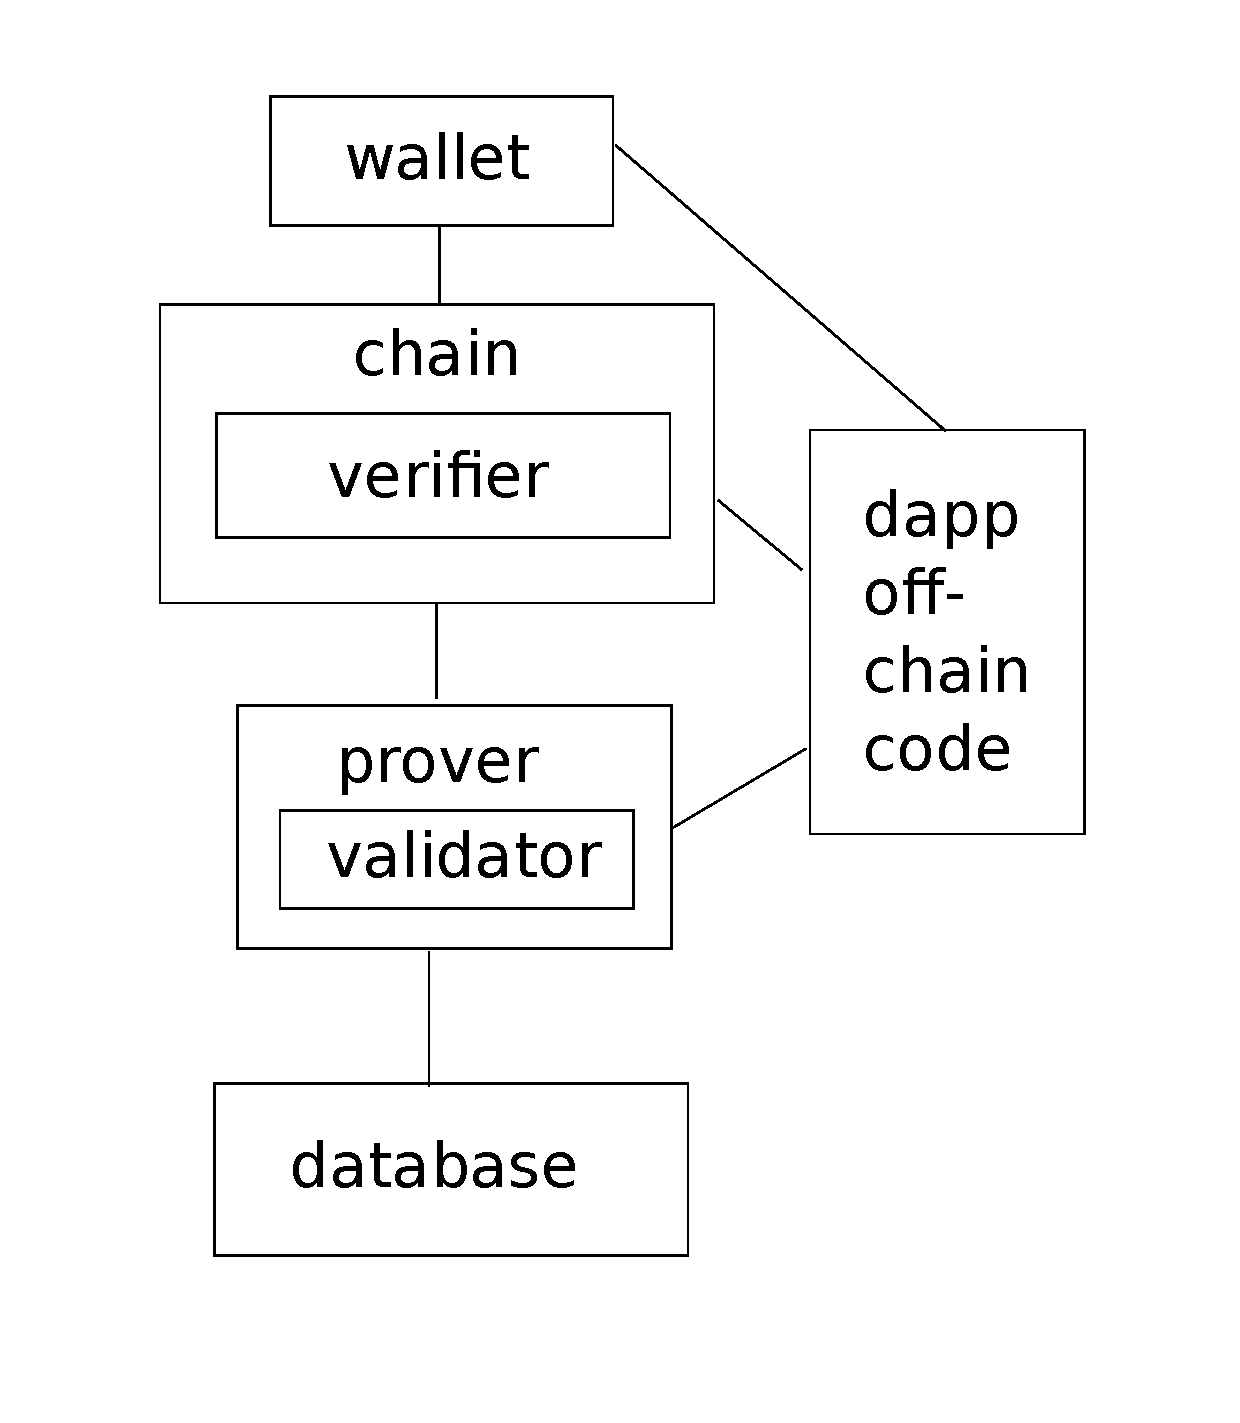
\includegraphics[width=1.0\columnwidth]{system-diagram.pdf}
	\caption{Key components of and related to Ardana Rollups.}
	\label{fig:system-diagram}
\end{figure}

Ardana Rollups provide an off-chain context in which smart contract validator code can run. Instead of being run to create transactions on the chain, in this context validator code is run to create transactions on the rollup and proofs that those transactions belong on the rollup.

It is important to keep two terms distinct here: \emph{verifier}\/ and \emph{validator}. ``Validator'' refers to a function which takes as input a transaction and produces as output a boolean value indicating whether or not the transaction satisfies the rules of a smart contract. ``Verifier'' refers to the smart contract validator which validates transactions over the rollup smart contract. The verifier is a validator, but other validators are not verifiers. In order to avoid confusion, let the term ``validator'' refer to the validator for some smart contract running on the rollup, as opposed to referring to the verifier (which runs on the blockchain).

Using Ardana Rollups complicates the process of developing a dapp (decentralized application) somewhat. The dapp must be aware of and control the movement of information from the chain to the rollup and back again. It must publish and subscribe to data not only on the chain but also on the rollup. The dapp interacts with the rollup by calling the prover API. The next section covers the processes involved in more detail.


\section{Processes}

There are three main processes involved in a dapp using Ardana Rollups: moving inputs from the chain to the rollup, posting transactions on the rollup, and moving outputs from the rollup to the chain. These processes are pictured in Figures~\ref{fig:process-a}, \ref{fig:process-b}, and \ref{fig:process-c}.

\begin{figure}
	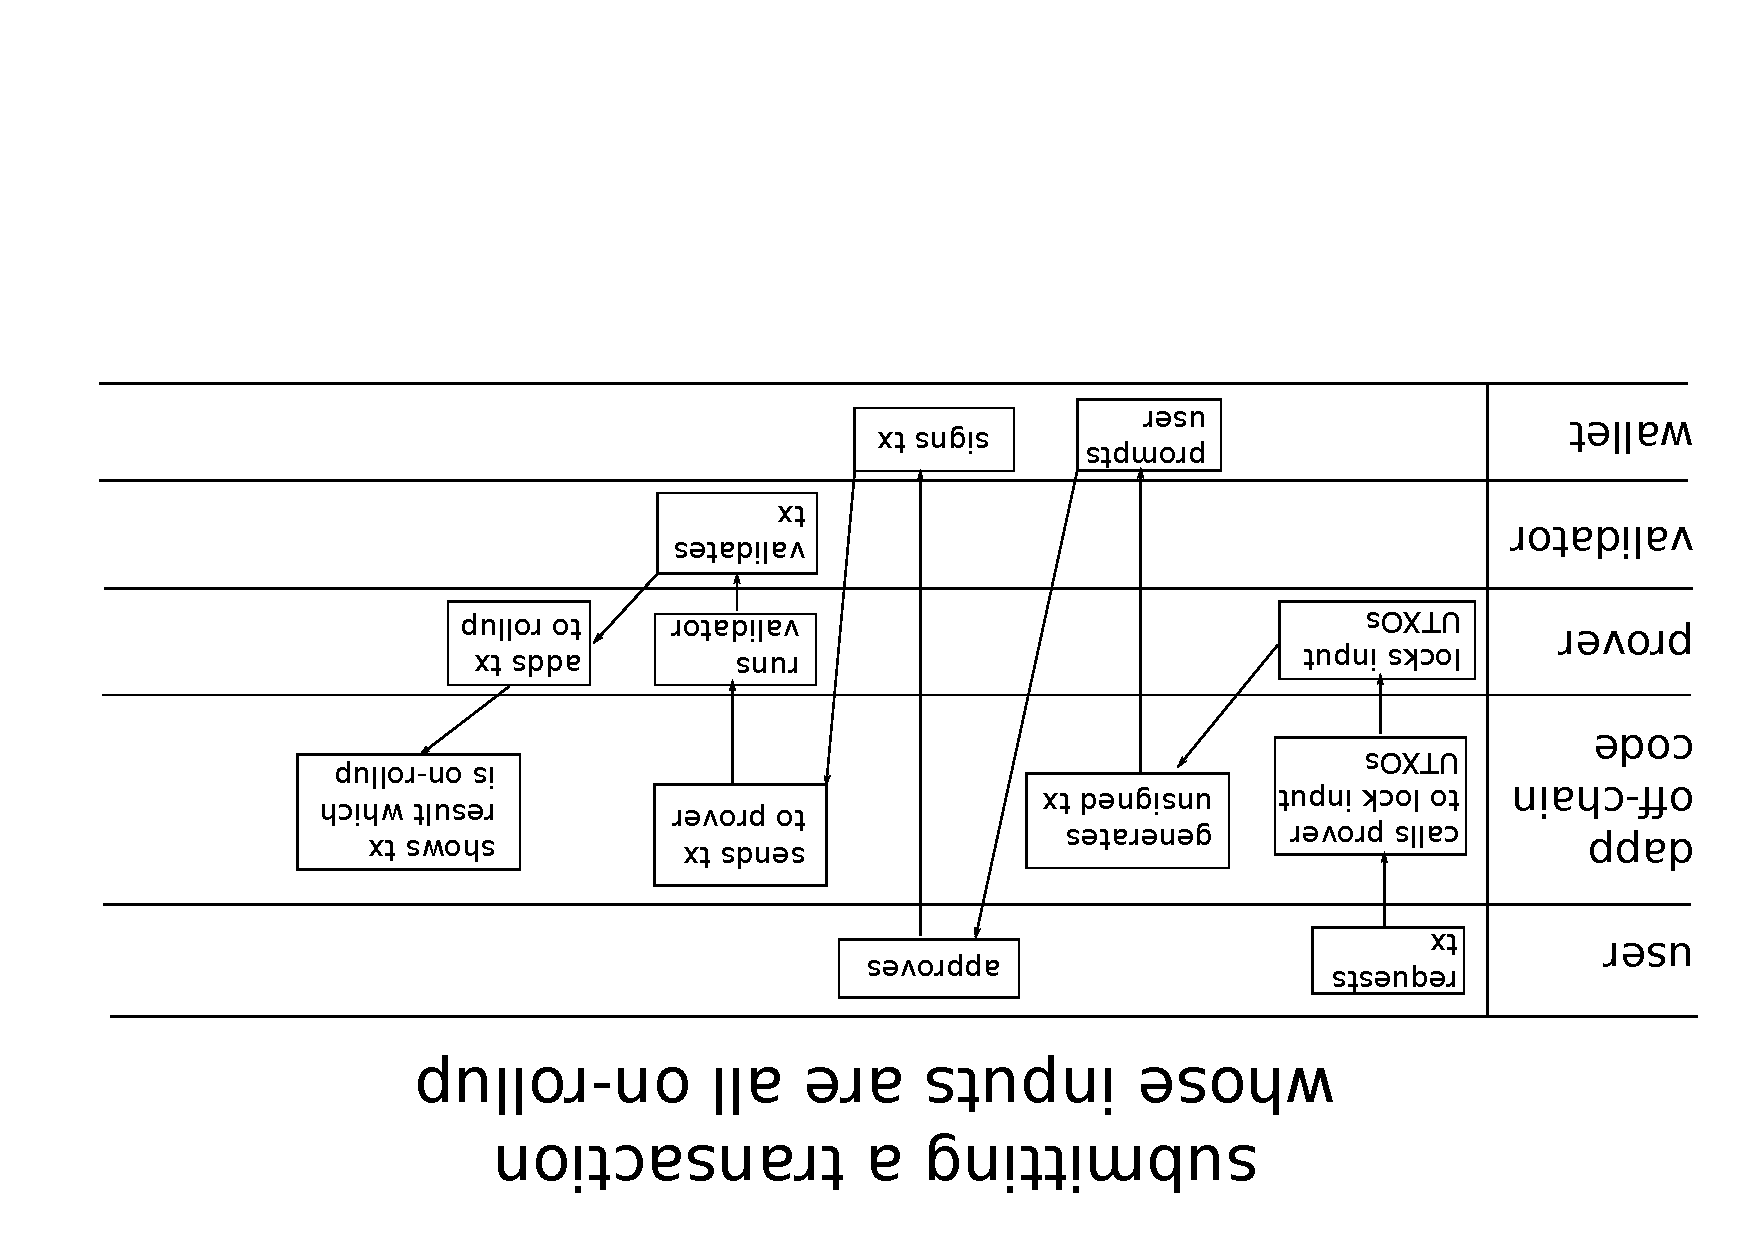
\includegraphics[angle=180,width=1.0\columnwidth]{process-diagram-a.pdf}
	\caption{Process of posting a transaction to a rollup.}
	\label{fig:process-a}
\end{figure}

\begin{figure}
	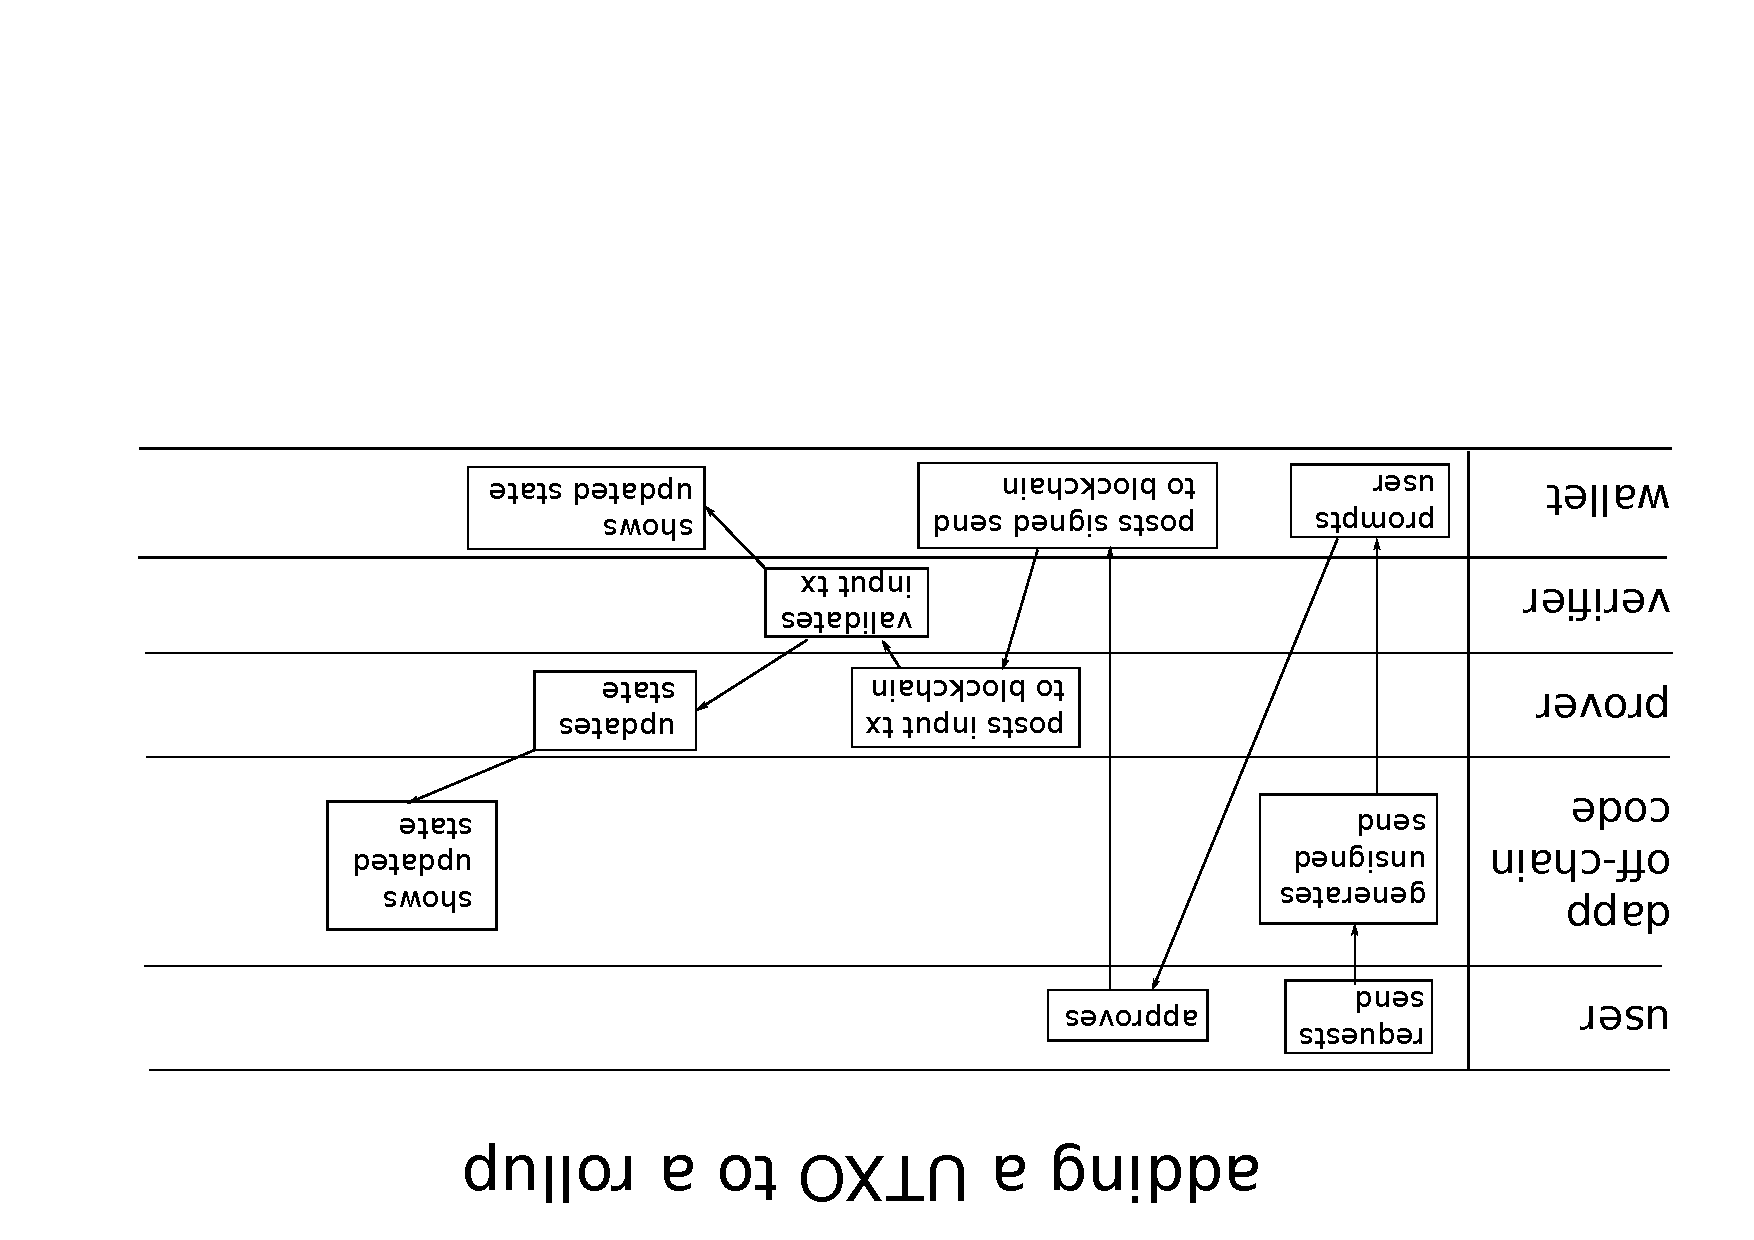
\includegraphics[angle=180,width=1.0\columnwidth]{process-diagram-b.pdf}
	\caption{Process of adding an input to a rollup.}
	\label{fig:process-b}
\end{figure}

\begin{figure}
	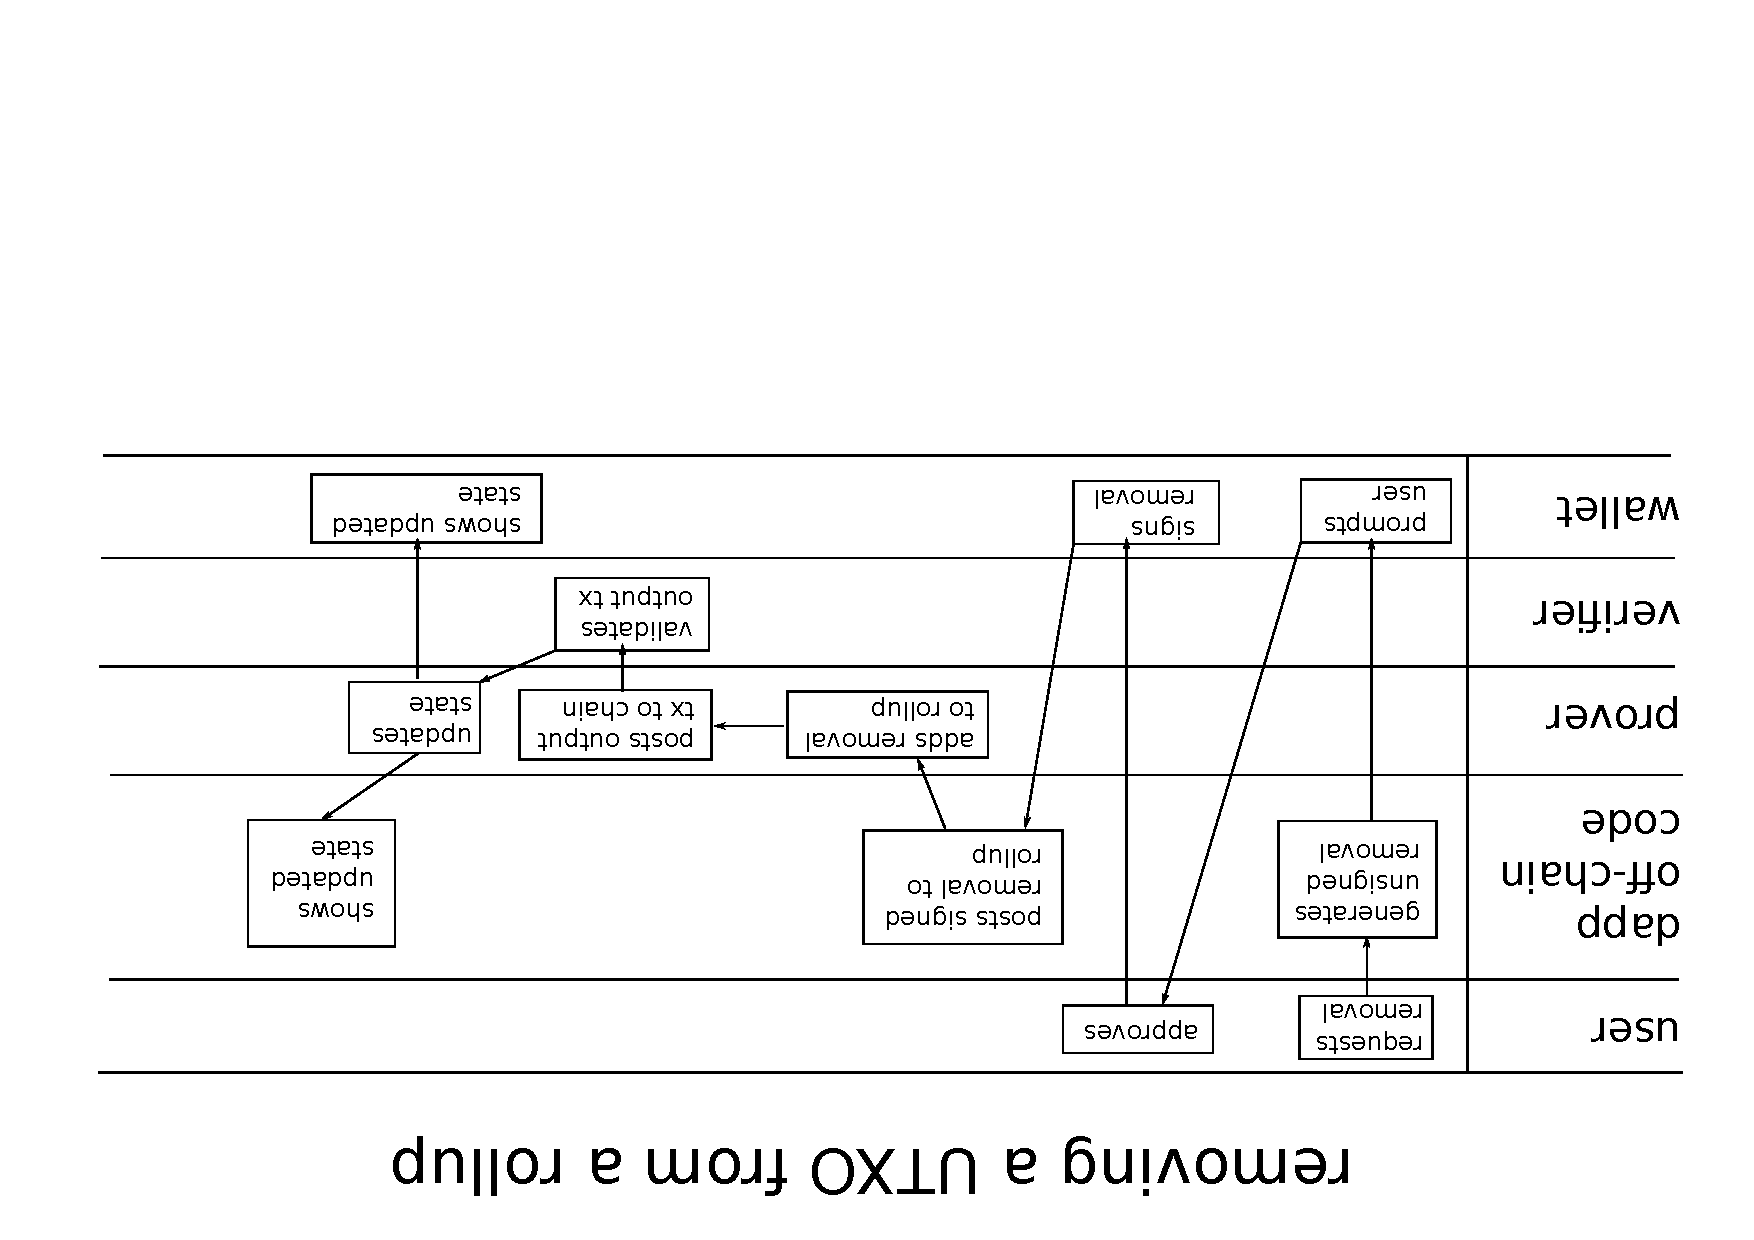
\includegraphics[angle=180,width=1.0\columnwidth]{process-diagram-c.pdf}
	\caption{Process of removing an output from a rollup.}
	\label{fig:process-c}
\end{figure}

\subsection{Process of posting a transaction to a rollup}

The first step of posting a transaction to a rollup is for the dapp code to call the prover API to lock the on-rollup input UTXOs. The purpose of this is to avoid resource contention problems which would prevent the transaction from going through. These locks should be temporary and expire automatically after a short time sufficient to complete the transaction. To avoid denial of service attacks based on this locking mechanism, the user requesting the transaction should be required to post collateral which will be lost if the locks expire without the inputs being used, or some other means should be used to prevent denial of service attacks based on this mechanism. The collateral can, for example, be one of the inputs being locked. Every transaction will have some monetary input, at least what is required to cover the transaction fee charged by the prover in order to cover the costs of proof generation. In response to the locking request, the prover provides some sort of key which the dapp may use to consume the on-rollup inputs. 

The next step is for the dapp to generate an unsigned transaction. The dapp sends the unsigned transaction to the user's wallet to be signed. The wallet signs the transaction with the user's approval. The dapp receives the signed transaction from the wallet and posts the transaction to the rollup by calling the prover API. The prover runs any validator scripts required for the transaction and generates a proof. The transaction, its outputs, and the proof are added to the rollup and the on-rollup inputs are marked as consumed. The dapp observes the rollup state changes via the prover API and makes them visible to the user.


\subsection{Process of adding an input to a rollup}

Adding an on-chain input to a rollup is essentially a two step process. First, the user sends the input to the rollup contract address. Second, the input gets picked up by an input transaction. The input transaction is an on-chain transaction which takes as input the rollup state UTXO and the inputs at the contract address which are to be added. It produces as output the new rollup state UTXO. The input transaction is signed by the prover. The rollup state UTXO contains the monetary values added to the rollup (in aggregate form, without tracking who owns what). It also contains whatever state data must be stored on-chain for the rollup contract.

Here is a speculative, non-binding description of what state data must be stored in the rollup UTXO. First, a nonce which gets incremented on every output transaction (described in the next section). Second, a hash of all of the on-rollup UTXOs. The mentioned hash may be a recursive hash, i.e. a hash of UTXOs and a previous hash. The purpose of the nonce is to help ensure that on-rollup UTXOs are not used more than once. The purpose of the state hash is to serve as an input to the proof checking algorithm.


\subsection{Process of removing an output from a rollup}

Removing an on-rollup output from the rollup and putting it on the chain is essentially a two step process. First, the user posts a removal transaction to the rollup. Second, the prover posts a removal transaction to the chain and updates its internal state. A removal transaction describes a set of output UTXOs and a proof (checked by the verifier contract) which shows that those outputs are lawful.


\section{Money trap avoidance}


\clearpage


\begin{thebibliography}{3}


	\bibitem{ethworks-20}
		Ethworks. \textit{Zero-Knowledge Blockchain Scalability}. Ethworks Reports, 2020. \url{https://ethworks.io/assets/download/zero-knowledge-blockchain-scaling-ethworks.pdf}

	\bibitem{visa}
		Visa. \textit{Power your retail business beyond the point of sale.} Accessed December 17, 2021. \url{https://usa.visa.com/run-your-business/small-business-tools/retail.html}

	\bibitem{chainweb}
		Will Martino, Monica Quaintance, and Stuart Popejoy. \textit{Chainweb: A Proof-of-Work Parallel-Chain Architecture for Massive Throughput.} DRAFT v15. \url{https://d31d887a-c1e0-47c2-aa51-c69f9f998b07.filesusr.com/ugd/86a16f_029c9991469e4565a7c334dd716345f4.pdf}


\end{thebibliography}



\end{document}
